% Options for packages loaded elsewhere
\PassOptionsToPackage{unicode}{hyperref}
\PassOptionsToPackage{hyphens}{url}
\PassOptionsToPackage{dvipsnames,svgnames,x11names}{xcolor}
%
\documentclass[
  11pt,
]{article}
\usepackage{amsmath,amssymb}
\usepackage[]{mathpazo}
\usepackage{iftex}
\ifPDFTeX
  \usepackage[T1]{fontenc}
  \usepackage[utf8]{inputenc}
  \usepackage{textcomp} % provide euro and other symbols
\else % if luatex or xetex
  \usepackage{unicode-math}
  \defaultfontfeatures{Scale=MatchLowercase}
  \defaultfontfeatures[\rmfamily]{Ligatures=TeX,Scale=1}
\fi
% Use upquote if available, for straight quotes in verbatim environments
\IfFileExists{upquote.sty}{\usepackage{upquote}}{}
\IfFileExists{microtype.sty}{% use microtype if available
  \usepackage[]{microtype}
  \UseMicrotypeSet[protrusion]{basicmath} % disable protrusion for tt fonts
}{}
\makeatletter
\@ifundefined{KOMAClassName}{% if non-KOMA class
  \IfFileExists{parskip.sty}{%
    \usepackage{parskip}
  }{% else
    \setlength{\parindent}{0pt}
    \setlength{\parskip}{6pt plus 2pt minus 1pt}}
}{% if KOMA class
  \KOMAoptions{parskip=half}}
\makeatother
\usepackage{xcolor}
\usepackage[margin = 1in]{geometry}
\usepackage{graphicx}
\makeatletter
\def\maxwidth{\ifdim\Gin@nat@width>\linewidth\linewidth\else\Gin@nat@width\fi}
\def\maxheight{\ifdim\Gin@nat@height>\textheight\textheight\else\Gin@nat@height\fi}
\makeatother
% Scale images if necessary, so that they will not overflow the page
% margins by default, and it is still possible to overwrite the defaults
% using explicit options in \includegraphics[width, height, ...]{}
\setkeys{Gin}{width=\maxwidth,height=\maxheight,keepaspectratio}
% Set default figure placement to htbp
\makeatletter
\def\fps@figure{htbp}
\makeatother
\setlength{\emergencystretch}{3em} % prevent overfull lines
\providecommand{\tightlist}{%
  \setlength{\itemsep}{0pt}\setlength{\parskip}{0pt}}
\setcounter{secnumdepth}{-\maxdimen} % remove section numbering
\newlength{\cslhangindent}
\setlength{\cslhangindent}{1.5em}
\newlength{\csllabelwidth}
\setlength{\csllabelwidth}{3em}
\newlength{\cslentryspacingunit} % times entry-spacing
\setlength{\cslentryspacingunit}{\parskip}
\newenvironment{CSLReferences}[2] % #1 hanging-ident, #2 entry spacing
 {% don't indent paragraphs
  \setlength{\parindent}{0pt}
  % turn on hanging indent if param 1 is 1
  \ifodd #1
  \let\oldpar\par
  \def\par{\hangindent=\cslhangindent\oldpar}
  \fi
  % set entry spacing
  \setlength{\parskip}{#2\cslentryspacingunit}
 }%
 {}
\usepackage{calc}
\newcommand{\CSLBlock}[1]{#1\hfill\break}
\newcommand{\CSLLeftMargin}[1]{\parbox[t]{\csllabelwidth}{#1}}
\newcommand{\CSLRightInline}[1]{\parbox[t]{\linewidth - \csllabelwidth}{#1}\break}
\newcommand{\CSLIndent}[1]{\hspace{\cslhangindent}#1}
\usepackage{setspace}\doublespacing
\ifLuaTeX
  \usepackage{selnolig}  % disable illegal ligatures
\fi
\IfFileExists{bookmark.sty}{\usepackage{bookmark}}{\usepackage{hyperref}}
\IfFileExists{xurl.sty}{\usepackage{xurl}}{} % add URL line breaks if available
\urlstyle{same} % disable monospaced font for URLs
\hypersetup{
  pdftitle={Dynamic Prediction of Non-Guassian Outcome with fast Generalized Functional Principal Analysis},
  pdfauthor={Ying Jin; Andrew Leroux},
  colorlinks=true,
  linkcolor={blue},
  filecolor={Maroon},
  citecolor={Blue},
  urlcolor={Blue},
  pdfcreator={LaTeX via pandoc}}

\title{Dynamic Prediction of Non-Guassian Outcome with fast Generalized
Functional Principal Analysis}
\author{Ying Jin \and Andrew Leroux}
\date{March 14, 2023}

\begin{document}
\maketitle

\hypertarget{introduction}{%
\section{Introduction}\label{introduction}}

Biomedical investigators are often interested in predicting future
observations of subjects based on their historical data, typically
referred to as dynamic prediction. Traditionally, this type of data has
been modeled using marginal models (generalized estimating equations) or
conditional models (mixed effect models)
(\protect\hyperlink{ref-Laird1982}{Laird and Ware 1982};
\protect\hyperlink{ref-liang1986}{LIANG and ZEGER 1986};
\protect\hyperlink{ref-lindstrom1990}{Lindstrom and Bates 1990};
\protect\hyperlink{ref-davidian2003}{{``Nonlinear models for repeated
measurement data''} 2003}), and predictions are made based on the
correlation between repeated measures from the same subject, and/or
covariates that can be either fixed or time-varying. However, these
methods are limited in terms of flexibility of correlation structure and
the ability to handle out-of-sample prediction. When sample size is
large or the density of repeated measures is high, they also tend to
cause severe computational burden
(\protect\hyperlink{ref-GLMMadaptive}{Rizopoulos 2022}).

To address these problems, one may turn to functional mixed effect
models instead when measures are dense across the domain. Such methods
accommodate more flexible correlation structure by modeling
subject-specific random effects as a function, and non-parametric
smoothing (\protect\hyperlink{ref-Scheipl2014}{Scheipl et al. 2014}) can
be incorporated to speed up the computation, such as spline basis
functions or eigenfunctions from functional principal component analysis
(fPCA). The introduction of basis functions also makes out-of-sample
prediction more straightforward. Instead of estimating subject-specific
random effects of new observations, we can simply estimate
coefficients/loadings on the basis function used for smoothing. Existing
research on dynamic prediction with functional data analysis methods has
been focusing on continuous/Gaussian outcomes, modelling
subject-specific random effects with FPCA
(\protect\hyperlink{ref-chiou2012}{Chiou 2012};
\protect\hyperlink{ref-goldberg2014}{Goldberg et al. 2014};
\protect\hyperlink{ref-shang2017}{Shang 2017}). Kraus
(\protect\hyperlink{ref-kraus2015}{2015}) has used this approach to
predict missing observations in partially observed function tracks, and
Delaigle and Hall (\protect\hyperlink{ref-delaigo2016}{2016}) achieved
similar goals using Markov Chains. While methods mentioned above used
only partial observations for prediction with an intercept-only model,
Leroux et al. (\protect\hyperlink{ref-leroux2016}{2018}) proposed
Functional Concurrent Regression (FCR) framework which can incorporate
the effect of subject-specific predictors. However, little extension was
made on prediction of non-Gaussian functions, such as binary and count
outcomes.

Unfortunately, fewer papers have focused on its extension to
non-Gaussian data, such as series of binary or count outcomes. Existing
methods also tend to be very computationally intensive. For example,
Chen et al. (\protect\hyperlink{ref-chen2013}{2013}) proposed approaches
to fit marginal functional models that is compatible to multi-level,
generalized outcomes. Goldsmith et al.
(\protect\hyperlink{ref-goldsmith2015}{2015}) established a model
framework that takes into account the fixed effect of time-invariant
covariates, with parameters estimated with Bayesian method in
\emph{Stan}. Gertheiss et al.
(\protect\hyperlink{ref-gertheiss2016}{2016}) identified bias introduced
by directly applying FPCA methods to generalized functions, and proposed
to address this problem using a two-stage, joint estimation strategy.
Linde (\protect\hyperlink{ref-linde2019}{2009}) used an adapted Bayesian
variational algorithm for FPCA of binary and count data. In terms of
implementation, Wrobel et al. (\protect\hyperlink{ref-wrobel2019}{2019})
proposed a fast, efficient way to fit GFPCA on binary data using EM
algorithm, accompanied by the an open source R package \emph{registr}.

In this paper, we aim to develop a fast, scalable method for dynamic
prediction of discrete function tracks based on functional mixed effect
model with fPCA smoothing. Section 2 presents the procedure of the
proposed method. In Section 3, we illustrate the performance and
efficiency of our proposed method in a simulation study. In Section 4,
we apply this method to a real-world dataset. Section 5 presents a
discussion of davantages and limitation of the proposed method.

\hypertarget{method}{%
\section{Method}\label{method}}

The observed data for a single subject \(i\) is (\(t\), \(Y_i(t)\)),
where \(t\) consists of dense, discrete points along the functional
domain, and \(Y_i(t)\) is the non-Gaussian outcome observed at \(t\). We
assume that the outcome \(Y_i(t)\) can be characterized by a latent
continuous function \(\eta_i(t)\). That is, at a specific t, \(Y_i(t)\)
follows a exponential family distribution such that:

\[
g[E(Y_i(t))] = \eta_i(t) = \beta_0(t)+b_i(t)
\]

where g is a appropriate link function, \(\beta_0(t)\) is the population
mean of latent function, and \(b_i(t)\) is a subjects-level random
effect function follows a zero-mean Gaussian process.

While \(b_i(t)\) is not observed, it can be approximated under the FPCA
framework \(b_i(t)=\sum_{k=1}^K\xi_{ik}\phi_{ik}(t)+\epsilon_i(t)\).
Here \(\phi_{ik}(t)\) is a set of orthogonal eigenfunctions that
explains the most variation in \(b_i(t)\), and \(\xi_{ik}\) are
subject-specific PC scores (or loadings) on each eigenfunction.
Additionally, \(\xi_{ik}\) are mutually independent obver both subject
(\(i\)) and eigenfunctions (\(k\)). That is, each \(\xi_{ik}\) follows
normal distribution \(N(0, \lambda_k)\) where \(\lambda_k\) is the kth
eigenvalues: \(\int \phi_k^2(t)dt=\lambda_k\). \(\epsilon_i(t)\) here is
a residual function that accounts for the variation not explained by the
first K eigenfunctions from FPCA. We assume it follows a zero-mean
Gaussian process. At a specific point t,
\(\epsilon_i(t) \sim N(0, \sigma^2)\).

Based on the problem set up above, we propose the following algorithm
for PFCA on the unobserved latent process \(\eta_i(t)\):

\begin{enumerate}
\def\labelenumi{\arabic{enumi}.}
\tightlist
\item
  Bin the observed outcomes in to small, non-overlapping, equal length
  intervals. We hereafter index the bins by their midpoints \(s\).
\item
  Fit a local Generalized Mixed Model at every bin. Specifically, at bin
  \(s\), we fit \(g[E(Y_i(t))] = \beta_0(s)+b_i(s)\) for all \(t\) in
  bin \(s\). From this series of models we can get estiamtes of
  population mean \(\hat{\beta}_0(s)\) and subject-level random effect
  \(\hat{b}_i(s)\), thus estimate of the individual latent functions at
  every bin: \(\hat{\eta}_i(s) = \hat{\beta}_0(s)+\hat{b}_i(s)\).
\item
  Fit FPCA on the estimated latent functions \(\hat{\eta}_i(s)\), and
  obtain estimates of basis functions
  \(\boldsymbol{\Phi} = \{\phi_1(s), ...,\phi_k(s)\}\), eigenvalues
  \(\hat{\lambda}_1...\hat{\lambda}_k\), population mean
  \(\hat{\beta}_0(s)\) and residual variance \(\hat{\sigma}^2\).
\item
  With components extracted above, calculate the maximum likelihood
  estimate (MLE) of the subject-specific PC scores \(\hat{\xi}_{ik}\) of
  new samples based on their partially observed data. Then the value of
  latent functions at unobserved points can be estimated as
  \(\hat{\eta_i}(s)=\hat{\beta}_0(s)+\sum_{k=1}^K\hat{\xi}_{ik}{\phi}_k(s)\)
\end{enumerate}

Following the algorithm above, predictions of individual latent
functions are made on the binned grid based on partially observed
non-Gaussian functions tracks of new subjects. Since the bins are set up
to be small in length, the binned grid would still be dense enough.
However, in situations where we need predictions on the original,
un-binned grid instead, linear interpolation turns out to be a fast,
convenient way with good performance for prediction at points between
bins.

Precision of prediction, usually quantified by the variance of
prediction error \(Var(\hat{\eta_i}(s)-\eta_i(s))\), is also
straightforward under this framework. In step 4 we calculated the MLE of
\(\hat{\xi}_{ik}\). Based on likelihood theory, its variance can be
estimated with observed information \({I}(\hat{\xi}_{ik})\), which is
essentially the second derivative of likelihood at \(\hat{\xi}_{ik}\).
Therefore, the variation of prediction interval is:

\[Var(\hat{\eta_i}(s)-\eta_i(s))=\boldsymbol{\Phi}(s)I(\hat{\boldsymbol{\xi}}_i)\boldsymbol{\Phi}^T(s)+\hat{\sigma_{\epsilon}}^2\]
Where \(\boldsymbol{\Phi}(s)=(\phi_1(s)...\phi_K(s))\) and
\(\hat{\boldsymbol{\xi}}_i=(\hat{\xi}_{i1}, ...,\hat{\xi}_{iK})\).

\hypertarget{simulation}{%
\section{Simulation}\label{simulation}}

In this section, we illustrate the predictive performance and
computational efficiency of the proposed method through a simulation
study. We simulated 50 datasets, each with 500 subjects. For every
subject, we generate 1000 binary outcomes \(Y_i(t) \in (0, 1)\) across
functional domain \(t \in [0, 1]\), where the distribution of outcome is
characterized by a continuous latent function. The data generation
mechanism can be expressed as follows:

\[\begin{aligned}
Y_i(t) & \sim Binomial(\frac{exp(\eta_i(t))}{1+exp(\eta_i(t))}) \\
\eta_i(t) &= f_0(t)+ \xi_{i1}sin(2\pi t)+\xi_{i2}cos(2\pi t)+\xi_{i3}sin(4\pi t)+\xi_{i4}cos(4\pi t)
\end{aligned}\]

In this simulation, we set \(f_0(t) = 0\). \(\xi_{ik}\) are mutually
independent normal random variables \(\xi_{ik}\sim N(0, \gamma_k)\).
Here we set the values of \(\gamma_k\) to be \(0.5^{k-1}\),
\(k \in (1,..., 4)\). In addition, for simplicity of presentation, we
generate data on a regular grid, which means observations points are
equally distributed across \([0, 1]\) and are the same for all subjects.

We use two metrics to evaluate the out-of-sample predictive performance:
integrated squared error (ISE) and
Area-Under-the-Receiver-Operator-Curve (AUC). ISE assess the prediction
accucay of latent continuous function. It is evaluated on the binned
grid at midpoints of each unobserved bin. If the entire functional
domian has S bins, but we have observations up to the mth bin, then ISE
is defined as
\(\frac{1}{N}\sum_{i=1}^N\sum_{s=m+1}^S(\hat{\eta}_i(s)-\eta_i(s))^2\).

The second metric, AUC, focuses on evaluation of prediction of the
binary outcome. Since the binary outcomes are generated on the original,
un-binned grid, we evaluated AUC on this grid as well and estimated
values of latent functions between bins with linear interpolation. Just
like ISE, the AUC report is also the average value across the whole
sample.

As a reference method, we compare our method to Generalized Linear Mixed
Models using Adaptive Gaussian Quadrature (GLMMadaptive). This is one of
the fastest existing method developed for dynamic prediction of repeated
generalized outcomes. Just like many mixed models, this method is very
limited in terms of flexibility. For example, the model used for
prediction of our simulated datset would simply be an linear model with
one covariate indicating observation time:
\(g(E(Y_i)) = \beta_0+\beta_1t+b_{i0}+b_{i1}t\). While the flexibility
of this mixed model can be increased using spline functions, the
dimension of spline basis is also restricted by computational ability,
and is unfeasible to implement under the scale of our simulated data or
the complexity of our proposed method.

\hypertarget{result}{%
\subsection{Result}\label{result}}

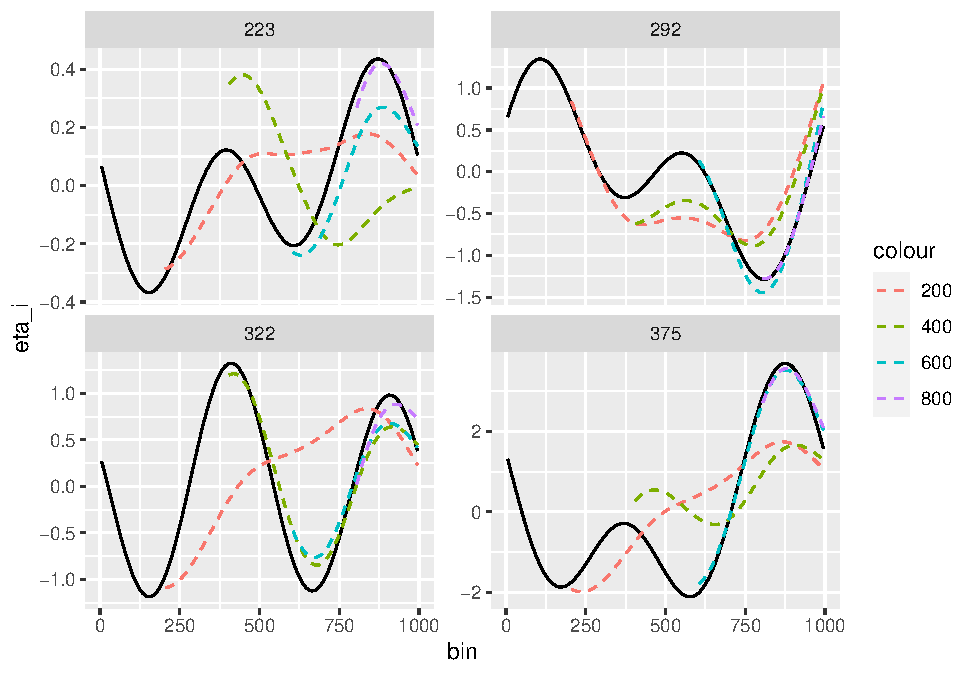
\includegraphics{Manuscript_files/figure-latex/unnamed-chunk-2-1.pdf}

\begin{verbatim}
## [1] 5.033985 5.134139 5.195642 5.152902 5.082466
\end{verbatim}

\hypertarget{data-application}{%
\section{Data application}\label{data-application}}

\hypertarget{discussion}{%
\section{Discussion}\label{discussion}}

\begin{itemize}
\tightlist
\item
  Grid
\item
  Score bias: cannot demonstrate without repeat simulation
\end{itemize}

\hypertarget{references}{%
\section{References}\label{references}}

\hypertarget{refs}{}
\begin{CSLReferences}{1}{0}
\leavevmode\vadjust pre{\hypertarget{ref-chen2013}{}}%
Chen, H., Wang, Y., Paik, M. cho, and Choi, H. A. (2013), {``A marginal
approach to reduced-rank penalized spline smoothing with application to
multilevel functional data,''} \emph{J Am Stat Assoc.}, 108, 1216--1229.
\url{https://doi.org/10.1080/01621459.2013.826134}.

\leavevmode\vadjust pre{\hypertarget{ref-chiou2012}{}}%
Chiou, J.-M. (2012), {``Dynamical functional prediction and
classification, with application to traffic flow prediction,''}
\emph{The Annals of Applied Statistics}, Institute of Mathematical
Statistics, 6, 1588--1614. \url{https://doi.org/10.1214/12-AOAS595}.

\leavevmode\vadjust pre{\hypertarget{ref-delaigo2016}{}}%
Delaigle, A., and Hall, P. (2016), {``Approximating fragmented
functional data by segments of markov chains,''} \emph{Biometrika}, 103,
779--799. \url{https://doi.org/10.1093/biomet/asw040}.

\leavevmode\vadjust pre{\hypertarget{ref-gertheiss2016}{}}%
Gertheiss, J., Goldsmith, J., and Staicu, A. (2016), {``A note on
modeling sparse exponential-family functional response curves,''}
\emph{Comput Stat Data Anal}, 105, 46--52.
\url{https://doi.org/10.1016/j.csda.2016.07.010}.

\leavevmode\vadjust pre{\hypertarget{ref-goldberg2014}{}}%
Goldberg, Y., Ritov, Y., and Mandelbaum, A. (2014), {``Predicting the
continuation of a function with applications to call center data,''}
\emph{Journal of Statistical Planning and Inference}, 147, 53--65.
https://doi.org/\url{https://doi.org/10.1016/j.jspi.2013.11.006}.

\leavevmode\vadjust pre{\hypertarget{ref-goldsmith2015}{}}%
Goldsmith, J., Zipunnikov, V., and Schrack, J. (2015), {``Generalized
multilevel function-on-scalar regression and principal component
analysis,''} \emph{Biometrics}, 71, 344--53.
\url{https://doi.org/10.1111/biom.12278}.

\leavevmode\vadjust pre{\hypertarget{ref-hall2018}{}}%
Hall, P., Müller, H.-G., and Yao, F. (2008), {``Modelling sparse
generalized longitudinal observations with latent gaussian processes,''}
\emph{Journal of the Royal Statistical Society: Series B (Statistical
Methodology)}, 70, 703--723.
https://doi.org/\url{https://doi.org/10.1111/j.1467-9868.2008.00656.x}.

\leavevmode\vadjust pre{\hypertarget{ref-kraus2015}{}}%
Kraus, D. (2015),
{``\href{http://www.jstor.org/stable/24775309}{Components and completion
of partially observed functional data},''} \emph{Journal of the Royal
Statistical Society. Series B (Statistical Methodology)}, {[}Royal
Statistical Society, Wiley{]}, 77, 777--801.

\leavevmode\vadjust pre{\hypertarget{ref-Laird1982}{}}%
Laird, N. M., and Ware, J. H. (1982),
{``\href{http://www.jstor.org/stable/2529876}{Random-effects models for
longitudinal data},''} \emph{Biometrics}, {[}Wiley, International
Biometric Society{]}, 38, 963--974.

\leavevmode\vadjust pre{\hypertarget{ref-leroux2022}{}}%
Leroux, A., Crainiceanu, C. M., and Wrobel, J. (n.d.). {``Fast
generalized functional principal component analysis.''}

\leavevmode\vadjust pre{\hypertarget{ref-leroux2016}{}}%
Leroux, A., Xiao, L., Crainiceanu, C., and Checkley, W. (2018),
{``Dynamic prediction in functional concurrent regression with an
application to child growth,''} \emph{Statistics in medicine}, 37,
1376--1388.

\leavevmode\vadjust pre{\hypertarget{ref-liang1986}{}}%
LIANG, K.-Y., and ZEGER, S. L. (1986), {``Longitudinal data analysis
using generalized linear models,''} \emph{Biometrika}, 73, 13--22.
\url{https://doi.org/10.1093/biomet/73.1.13}.

\leavevmode\vadjust pre{\hypertarget{ref-linde2019}{}}%
Linde, van der (2009), {``A bayesian latent variable approach to
functional principal components analysi with binary and count data,''}
\emph{A StA Adv Stat Anal}, 307--333.
\url{https://doi.org/10.1007/s10182-009-0113-6}.

\leavevmode\vadjust pre{\hypertarget{ref-lindstrom1990}{}}%
Lindstrom, M. J., and Bates, D. M. (1990),
{``\href{http://www.jstor.org/stable/2532087}{Nonlinear mixed effects
models for repeated measures data},''} \emph{Biometrics}, {[}Wiley,
International Biometric Society{]}, 46, 673--687.

\leavevmode\vadjust pre{\hypertarget{ref-davidian2003}{}}%
{``\href{http://www.jstor.org/stable/1400665}{Nonlinear models for
repeated measurement data: An overview and update}''} (2003),
{[}International Biometric Society, Springer{]}, 8, 387--419.

\leavevmode\vadjust pre{\hypertarget{ref-GLMMadaptive}{}}%
Rizopoulos, D. (2022),
\emph{\href{https://CRAN.R-project.org/package=GLMMadaptive}{GLMMadaptive:
Generalized linear mixed models using adaptive gaussian quadrature}}.

\leavevmode\vadjust pre{\hypertarget{ref-Scheipl2014}{}}%
Scheipl, F., Staicu, A.-M., and Greven, S. (2014), {``Functional
additive mixed models,''} \emph{J Comput Graph Stat}, 24, 447--501.
\url{https://doi.org/10.1080/10618600.2014.901914}.

\leavevmode\vadjust pre{\hypertarget{ref-shang2017}{}}%
Shang, H. L. (2017), {``Functional time series forecasting with dynamic
updating: An application to intraday particulate matter
concentration,''} \emph{Econometrics and Statistics}, 1, 184--200.
https://doi.org/\url{https://doi.org/10.1016/j.ecosta.2016.08.004}.

\leavevmode\vadjust pre{\hypertarget{ref-suresh2017}{}}%
Suresh, K., Taylor, J. M. G., Spratt, D. E., Daignault, S., and
Tsodikov, A. (2017), {``Comparison of joint modeling and landmarking for
dynamic prediction under an illness-death model,''} \emph{Biom J}, 59,
1277--1300. \url{https://doi.org/10.1002/bimj.201600235}.

\leavevmode\vadjust pre{\hypertarget{ref-wrobel2019}{}}%
Wrobel, J., Zipunnikov, V., Schrack, J., and Goldsmith, J. (2019),
{``Registration for exponential family functional data,''}
\emph{Biometrics}, 75, 48--57.
https://doi.org/\url{https://doi.org/10.1111/biom.12963}.

\end{CSLReferences}

\end{document}
